\chapter{THIẾT KẾ QUAN NIỆM (ERD/EER)}

\section{Phương pháp luận áp dụng}

Áp dụng thuật toán thiết kế ER theo 7 bước: (1) khoanh phạm vi dữ liệu, (2) lập từ điển nghiệp vụ, (3) chọn thực thể/thuộc tính/khóa, (4) xác định mối kết hợp và bản số, (5) hỏi lại mức tham gia bắt buộc/tùy chọn, (6) kiểm chứng bằng dữ liệu mẫu, (7) chốt ERD/EER quan niệm.

\section{Danh sách thực thể và thuộc tính}

\begin{center}
\begin{tabularx}{\linewidth}{@{}l>{\raggedright\arraybackslash}X>{\raggedright\arraybackslash}X@{}}
\toprule
\textbf{Thực thể} & \textbf{Thuộc tính chính} & \textbf{Ghi chú} \\
\midrule
NguoiDung & maND (PK), email, matKhauHash, ngayTao & --- \\
GiaDinh & maGD (PK), tenGiaDinh, ngayTao & --- \\
ThanhVien & maTV (PK), hoTen, ngaySinh, ngayMat, gioiTinh, /tuoi & /tuoi là thuộc tính dẫn xuất từ ngaySinh \\
VaiTro & maVT (PK), tenVT & Dùng cho RBAC \\
BaiViet & maBV (PK), noiDung, ngayDang & --- \\
BinhLuan & maBV (FK) + sttBL (khóa cục bộ), noiDung, ngayBL & Thực thể yếu, phụ thuộc BaiViet \\
SuKien & maSK (PK), tenSK, diaDiem, ngayDienRa & --- \\
HoSoNgheNghiep & maHS (PK), ngheNghiep, noiCongTac, tuNam, denNam & Thực thể riêng vì lưu lịch sử nhiều nghề \\
TaiLieuLichSu & maTL (PK), tieuDe, loaiTepTin, url & --- \\
HonNhan & maHN (PK), maTV1 (FK), maTV2 (FK), ngayKetHon, ngayLyHon, trangThai & Association class tự thân trên ThanhVien \\
PhanQuyen & maND (FK), maGD (FK), maVT (FK) & Bảng trung gian RBAC; PK tổ hợp 3 khóa, không có thuộc tính riêng \\
NhatKyKiemToan & maNK (PK), maND (FK, NULL được), hanhDong, doiTuong, thoiGian & Ghi log CRUD phục vụ audit; maND NULL nếu hệ thống tự động thực hiện \\
\bottomrule
\end{tabularx}
\end{center}

\section{Mối kết hợp và bản số}

Đây là phần trọng tâm của mô hình vì gia phả có bản chất là đồ thị tự tham chiếu trên chính thực thể ThanhVien:

\begin{center}
\begin{tabularx}{\linewidth}{@{}>{\raggedright\arraybackslash}p{3.6cm}l>{\raggedright\arraybackslash}X@{}}
\toprule
\textbf{Mối kết hợp} & \textbf{Bản số} & \textbf{Ghi chú thiết kế} \\
\midrule
GiaDinh --- ThanhVien & 1 : N & ThanhVien nhận khóa ngoại maGD \\
NguoiDung --- ThanhVien & 0..1 : 0..1 & 1:1 tùy chọn; FK đặt ở NguoiDung, ràng buộc UNIQUE \\
ThanhVien --- ThanhVien (QuanHeChaCon) & N : N (tự thân), có thuộc tính vaiTro & Mối kết hợp có thuộc tính riêng → bảng trung gian \\
ThanhVien --- ThanhVien (HonNhan) & N : N (tự thân), có thuộc tính ngày/trạng thái & Association class riêng do có thể nhiều lần kết hôn \\
BaiViet --- BinhLuan & 1 : N & BinhLuan là thực thể yếu \\
NguoiDung --- BaiViet & 1 : N & Người đăng bài \\
SuKien --- NguoiDung (ThamGiaSuKien) & M : N, có thuộc tính trangThai, ngayThamGia & Bảng trung gian \\
NguoiDung --- VaiTro --- GiaDinh (PhanQuyen) & M : N : N & RBAC theo ngữ cảnh từng gia đình \\
GiaDinh --- TaiLieuLichSu & 1 : N & --- \\
NguoiDung --- BinhLuan & 1 : N & Người viết bình luận (maND trong BinhLuan) \\
ThanhVien --- HoSoNgheNghiep & 1 : N & Lịch sử nghề nghiệp của thành viên \\
NguoiDung --- NhatKyKiemToan & 0..1 : N & Ghi log; maND NULL nếu do hệ thống tự động \\
\bottomrule
\end{tabularx}
\end{center}

\begin{figure}[htbp]
\centering
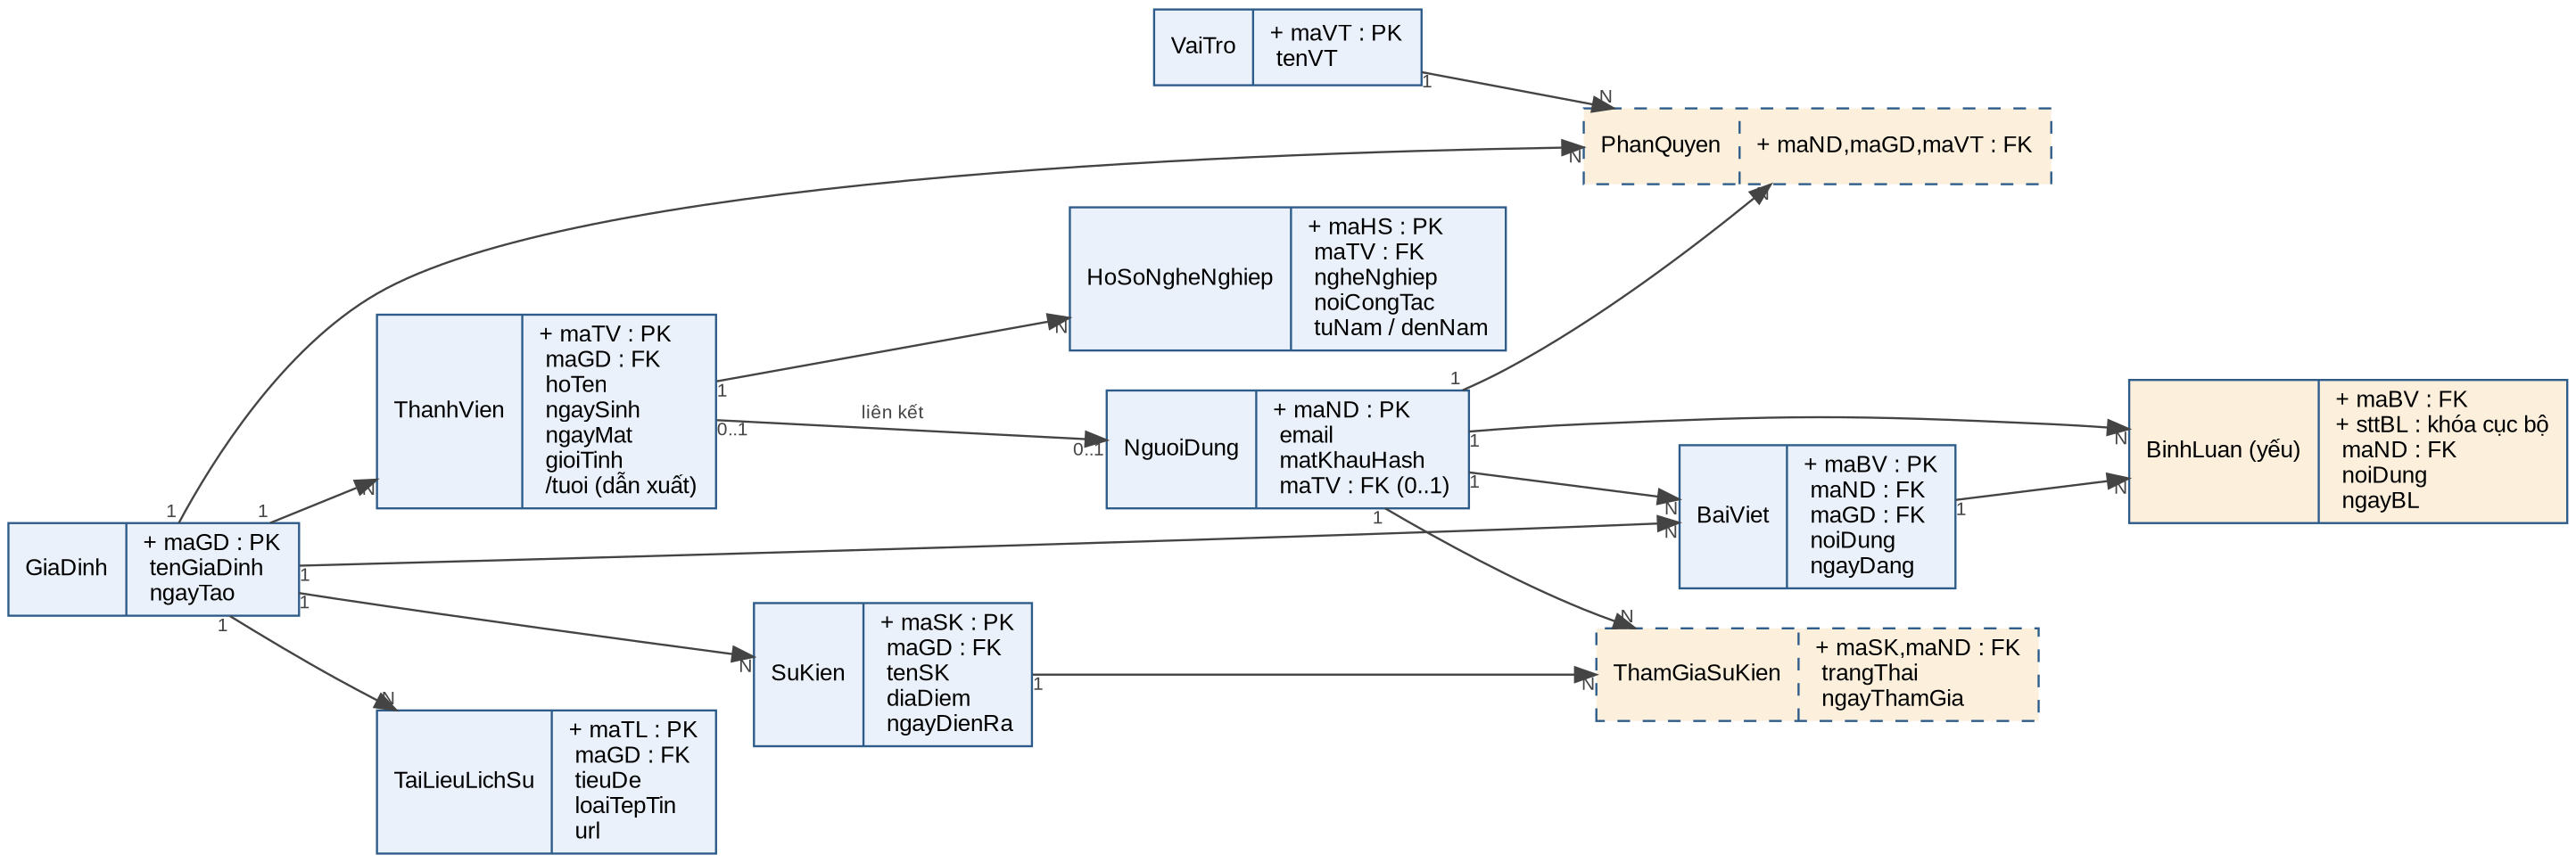
\includegraphics[width=0.95\linewidth]{images/erd_tongthe.png}
\caption{ERD tổng thể (ký pháp lớp UML: khối trên là thực thể, khối viền đứt là mối kết hợp có thuộc tính riêng)}
\end{figure}

\subsection*{Chi tiết mối kết hợp tự thân trên ThanhVien}
\addcontentsline{toc}{subsection}{Chi tiết mối kết hợp tự thân trên ThanhVien}

Vì quan hệ huyết thống và hôn nhân đều diễn ra giữa hai thể hiện của cùng một thực thể ThanhVien, cần tách rõ thành hai mối kết hợp độc lập để tránh nhầm lẫn khi chuyển sang lược đồ quan hệ:

\begin{figure}[htbp]
\centering
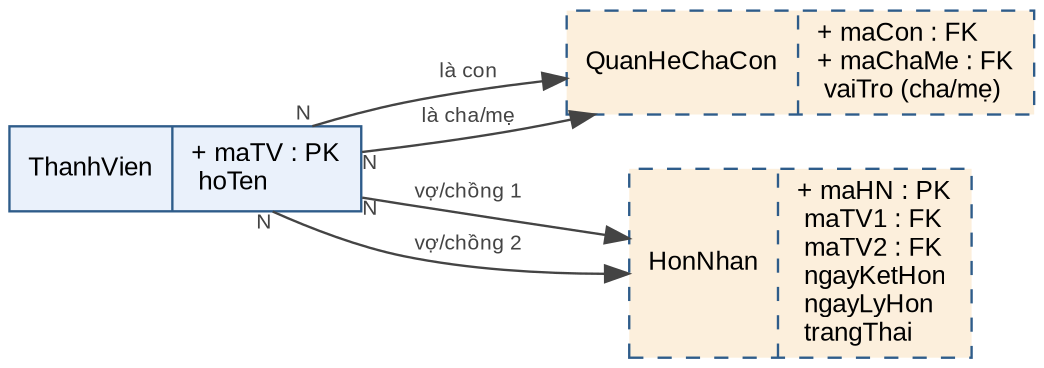
\includegraphics[width=0.75\linewidth]{images/erd_tuthanpk.png}
\caption{Mối kết hợp tự thân: QuanHeChaCon và HonNhan trên thực thể ThanhVien}
\end{figure}

\section{Đặc tả EER --- Chuyên biệt hóa tài khoản}

Hệ thống phân biệt hai dạng tài khoản theo mức quyền: Quản trị gia đình (được tạo/sửa cấu trúc gia phả) và Thành viên thường (chỉ xem/tương tác). Áp dụng chuyên biệt hóa \{disjoint, complete\}:

Ánh xạ chuyên biệt hóa này được đưa chính thức vào lược đồ quan hệ ở mục 4.1 (hai bảng QuanTriGiaDinh, ThanhVienThuong), thay vì chỉ dừng ở mức khái niệm.

\begin{infobox}
\begin{verbatim}
NguoiDung(maND, email, matKhauHash)
 +-- QuanTriGiaDinh(maND PK/FK, quyenDacBiet)
 `-- ThanhVienThuong(maND PK/FK)
\end{verbatim}
\end{infobox}

\section{Kiểm chứng bằng dữ liệu mẫu}

\begin{itemize}
  \item Thêm một ThanhVien chưa có tài khoản NguoiDung (thành viên đã mất, thế hệ trước) → mô hình vẫn hợp lệ nhờ bản số 0..1.
  \item Thêm một ThanhVien có 2 lần HonNhan tại hai thời điểm khác nhau → hợp lệ nhờ HonNhan là association class riêng, không gộp vào ThanhVien.
  \item Xóa một GiaDinh → cần xác định chính sách xóa (cascade hoặc chặn) cho ThanhVien, BaiViet, SuKien liên quan --- ghi chú này chuyển thành ràng buộc ON DELETE ở Chương 5.
\end{itemize}

